% EESC 4464/6664 — Data Lab #3, Part 2: The Blob
% Compile: pdflatex DataLab3_Part2_Report.tex (run twice if using cross-refs)
\documentclass[11pt,letterpaper]{article}

\usepackage[margin=1in]{geometry}
\usepackage{graphicx}
\usepackage{amsmath}
\usepackage{booktabs}
\usepackage{hyperref}
\usepackage{siunitx}
\usepackage{float}

\sisetup{detect-all}
\newcommand{\degC}{\si{\degreeCelsius}}

\title{Data Lab \#3, Part 2: Combining in situ, climatological, and satellite estimates of temperature anomalies at Ocean Station Papa}
\author{Your Name}
\date{April 2026}

\begin{document}
\maketitle

\begin{abstract}
Marine heatwaves such as the northeast Pacific event known as ``the Blob'' leave fingerprints in multiple observing systems that differ in depth, sampling, and processing. At Ocean Station Papa (OSP), I combined Ocean Observatories Initiative (OOI) CTD temperatures from Flanking Mooring B, World Ocean Atlas 2013 (WOA13) decadal climatology, and the JPL Multi-scale Ultra-high Resolution (MUR) \emph{monthly SST anomaly} product (NOAA CoastWatch ERDDAP subset, 2013--February~2020). The mooring anomaly removes the WOA seasonal cycle at \SI{30}{\meter}; the satellite field is a provider-computed anomaly relative to a MUR climatology (2003--2014). I compare the two point records and, in an extension, map regional SST anomaly for several months within the mooring overlap, marking those months on the time-series figure.
\end{abstract}

% ------------------------------------------------------------------
\section{Introduction}

\subsection*{Why marine heatwaves and the Blob matter}
The ocean absorbs most of the excess heat from anthropogenic radiative forcing, and episodic warm extremes superimposed on that background can reorganize ecosystems, fisheries, and biogeochemistry over large regions \cite{bond2015,hobday2016}. The northeast Pacific warm anomaly peaking around 2014--2016---often called the Blob---was associated with widespread SST anomalies, changes in primary production, and unusual occurrences along the west coast of North America \cite{bond2015}. Understanding such events requires observations that resolve both seasonal cycles and interannual anomalies, often from more than one platform because no single instrument samples all relevant scales.

\subsection*{Questions addressed in this analysis}
This report addresses three connected questions:
\begin{enumerate}
  \item How does near-surface temperature from the OOI mooring at OSP compare to the long-term mean seasonal cycle represented by WOA13 at the same location and depth?
  \item After removing that climatological seasonal cycle, what mooring-based temperature anomaly time series is obtained, and how does it compare to an SST anomaly estimate from satellite data at the nearest grid cell?
  \item How does the OSP record sit inside broader spatial patterns of SST anomaly on the satellite grid at selected times (extension)?
\end{enumerate}

\subsection*{Connection to the analysis}
The first question motivates overlaying OOI temperatures (quality-controlled in Part~1) on the repeated monthly WOA climatology (Figure~\ref{fig:woa_ooi}). The second motivates interpolating WOA to each good mooring time and forming anomalies, then comparing to satellite-based anomalies (Figure~\ref{fig:anomaly_compare}). The third uses the same satellite anomaly field to map several snapshots and mark those dates on the time series (Figure~\ref{fig:maps}), linking point anomalies to regional structure during the mooring record.

% ------------------------------------------------------------------
\section{Methods}

\subsection{Data sources}

\paragraph{OOI mooring CTD (in situ).}
Temperature comes from the GP03FLMB CTD on Ocean Observatories Initiative Flanking Mooring B near OSP ($\sim$\ang{50.1}\,N, \ang{144.9}\,W). Files are 15-minute resolution NetCDF deployments (0001, 0003--0006) accessed via the course data bundle (originally from the OOI Data Portal). The instrument reports \emph{in situ} temperature at a nominal depth near \SI{30}{\meter} (depth held fixed in this lab relative to WOA).

\paragraph{WOA13 climatology (gridded compilation).}
WOA13 provides objectively analyzed mean temperature on a \ang{1} horizontal grid and standard depth levels, here subset to the North Pacific \cite{locarnini2013}. I used variable \texttt{t\_an} (analyzed mean) for each calendar month. At OSP I selected the nearest grid indices for longitude, latitude, and a depth near \SI{30}{\meter} for comparison to the mooring.

\paragraph{Satellite SST anomaly (gridded remote sensing).}
I used a regional NetCDF extract of the JPL MUR monthly SST \emph{anomaly} product (variable \texttt{sstAnom}, \degC{}) on a $\sim$\SI{0.01}{\degree} grid, with time in POSIX seconds since 1970-01-01 \cite{chin2017}. According to the file metadata, each monthly field is the mean of daily MUR anomalies, where daily anomalies were formed by NOAA ERD using the JPL MUR climatology for 2003--2014. The subset spans January~2013 through February~2020 (86 monthly time steps), which aligns well with the OOI record used here.

\subsection{Processing the OOI record (Part~1 carryover)}
For each deployment, I converted OOI time from seconds since 1900-01-01 to MATLAB datenum. I computed a one-day moving mean and moving standard deviation (window sized using the \SI{15}{\minute} sample interval). Following Part~1, points where the moving standard deviation exceeded \SI{0.25}{\degreeCelsius} were excluded as ``bad'' intervals (likely biofouling, mechanical issues, or other high-noise periods). All Part~2 results use only indices labeled \texttt{good\_idx}.

\subsection{Mooring temperature anomaly relative to WOA}
The extended WOA timeline repeats the twelve monthly climatological values at OSP (\SI{30}{\meter}) across January~2013--March~2020 on the 15th of each month, matching the course template. I linearly interpolated that climatology to each retained mooring time $t_i$:
\begin{equation}
  T_{\mathrm{WOA,interp}}(t_i) = \mathrm{interp1}\bigl(t_{\mathrm{WOA}},\, T_{\mathrm{WOA,rep}},\, t_i,\, \text{linear}\bigr),
\end{equation}
where $t_{\mathrm{WOA}}$ is the vector of datenum times for the repeated monthly climatology, $T_{\mathrm{WOA,rep}}$ is the corresponding climatological temperature at OSP (\SI{30}{\meter}), and $\mathrm{interp1}$ denotes one-dimensional linear interpolation in MATLAB. The mooring anomaly is
\begin{equation}
  T'_{\mathrm{moor}}(t_i) = T_{\mathrm{OOI}}(t_i) - T_{\mathrm{WOA,interp}}(t_i),
\end{equation}
where $T_{\mathrm{OOI}}(t_i)$ is the quality-controlled mooring temperature at time $t_i$. Subscript ``moor'' indicates the in situ record; the prime denotes departure from the WOA seasonal climatology (not a pre-computed OISST anomaly product).

\subsection{Satellite SST anomaly}
\label{sec:sat_anom}
The NetCDF already supplies monthly $T'_{\mathrm{sat}}(x,y,t_k)$ as \texttt{sstAnom}. I used the nearest grid indices to OSP (same nearest-neighbor logic as for WOA) to form a time series $T'_{\mathrm{sat,OSP}}(t_k)$. For comparison at every good mooring time $t_i$, I linearly interpolated that monthly series:
\begin{equation}
  T'_{\mathrm{sat,interp}}(t_i) = \mathrm{interp1}\bigl(t_{\mathrm{sat}},\, T'_{\mathrm{sat,OSP}},\, t_i,\, \text{linear},\, \mathrm{NaN}\bigr),
\end{equation}
where $t_{\mathrm{sat}}$ is the vector of satellite sampling times (monthly). Equation~(3) is used only to place satellite and mooring records on a common time axis; it does not change the satellite provider's anomaly definition (MUR baseline 2003--2014), which differs from the WOA-based mooring anomaly in Equation~(2).

\subsection{Uncertainty and data quality}
Several sources of uncertainty affect interpretation:
\begin{itemize}
  \item \textbf{Representativeness:} Mooring temperature is at $\sim$\SI{30}{\meter}; satellite SST is a skin/foundation-temperature product. Vertical structure and diurnal cycles are not resolved the same way.
  \item \textbf{Climatology mismatch:} WOA13 is a long-term decadal mean with \ang{1} smoothing; it does not include interannual variability. Any warm or cool period relative to the 2010s will appear as ``anomaly'' in Equation~(2) even if it partly reflects climate drift or WOA baseline choice.
  \item \textbf{QC choices:} The \SI{0.25}{\degreeCelsius} moving-standard-deviation cutoff removes noisy segments but is subjective; different cutoffs would change which points enter Equation~(2).
  \item \textbf{Different anomaly baselines:} $T'_{\mathrm{moor}}$ uses WOA13; $T'_{\mathrm{sat}}$ uses the MUR 2003--2014 climatology. A constant offset or seasonal residual can appear even if both sensors track the same physical events.
  \item \textbf{Temporal sampling:} Satellite data are monthly means; the mooring is $\sim$\SI{15}{\minute} after QC. Sub-monthly variability appears only in Equation~(2).
\end{itemize}

% ------------------------------------------------------------------
\section{Results and discussion}

\begin{figure}[H]
  \centering
  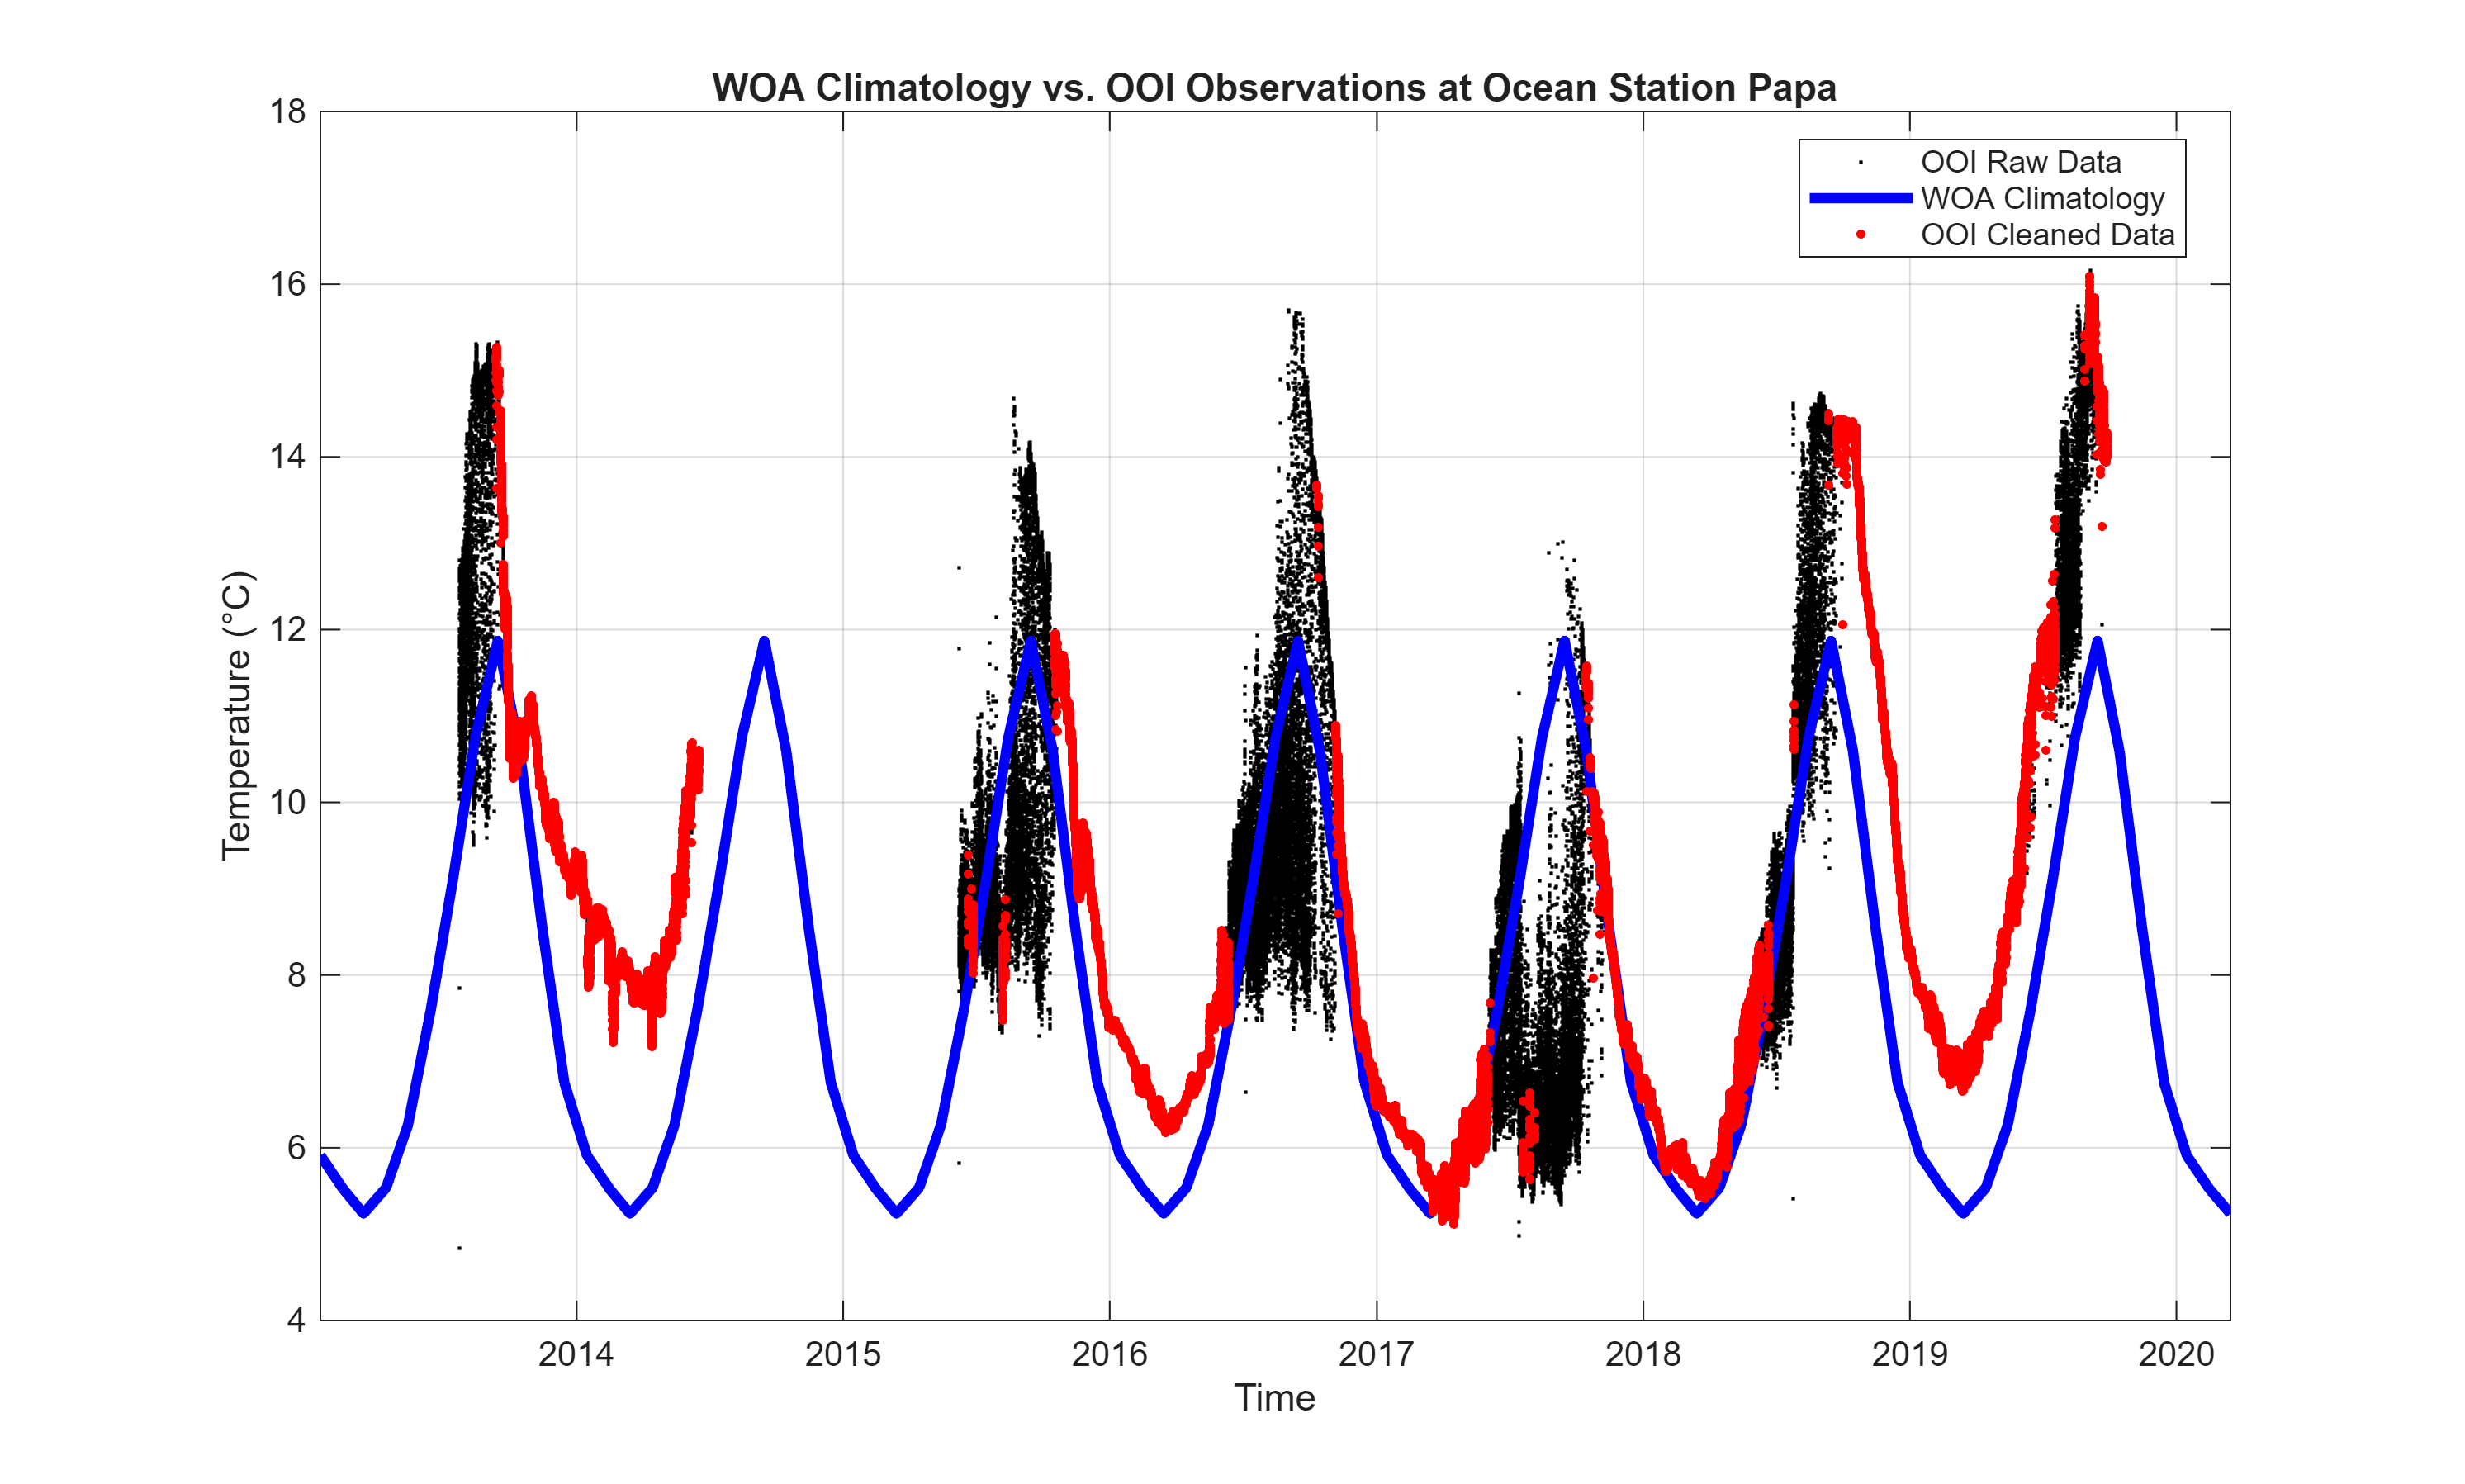
\includegraphics[width=0.95\textwidth]{figures/fig01_woa_ooi.png}
  \caption{WOA13 climatological temperature at Ocean Station Papa (\SI{30}{\meter}, repeated seasonal cycle, thick blue line) compared to all OOI Flanking Mooring B temperatures (small black points) and quality-controlled (``cleaned'') OOI points from Part~1 (red). The climatology repeats each calendar year; raw deployments show noise and gaps, while cleaned points emphasize intervals that passed the moving-standard-deviation screen.}
  \label{fig:woa_ooi}
\end{figure}

Figure~\ref{fig:woa_ooi} shows that OOI temperatures generally track the WOA seasonal cycle but depart substantially during warm periods (notably mid-decade) and show gaps when deployments end or data are rejected. The comparison makes clear that WOA describes a smoothed, long-term mean month-by-month field, while the mooring resolves weather-to-seasonal variability.

\begin{figure}[H]
  \centering
  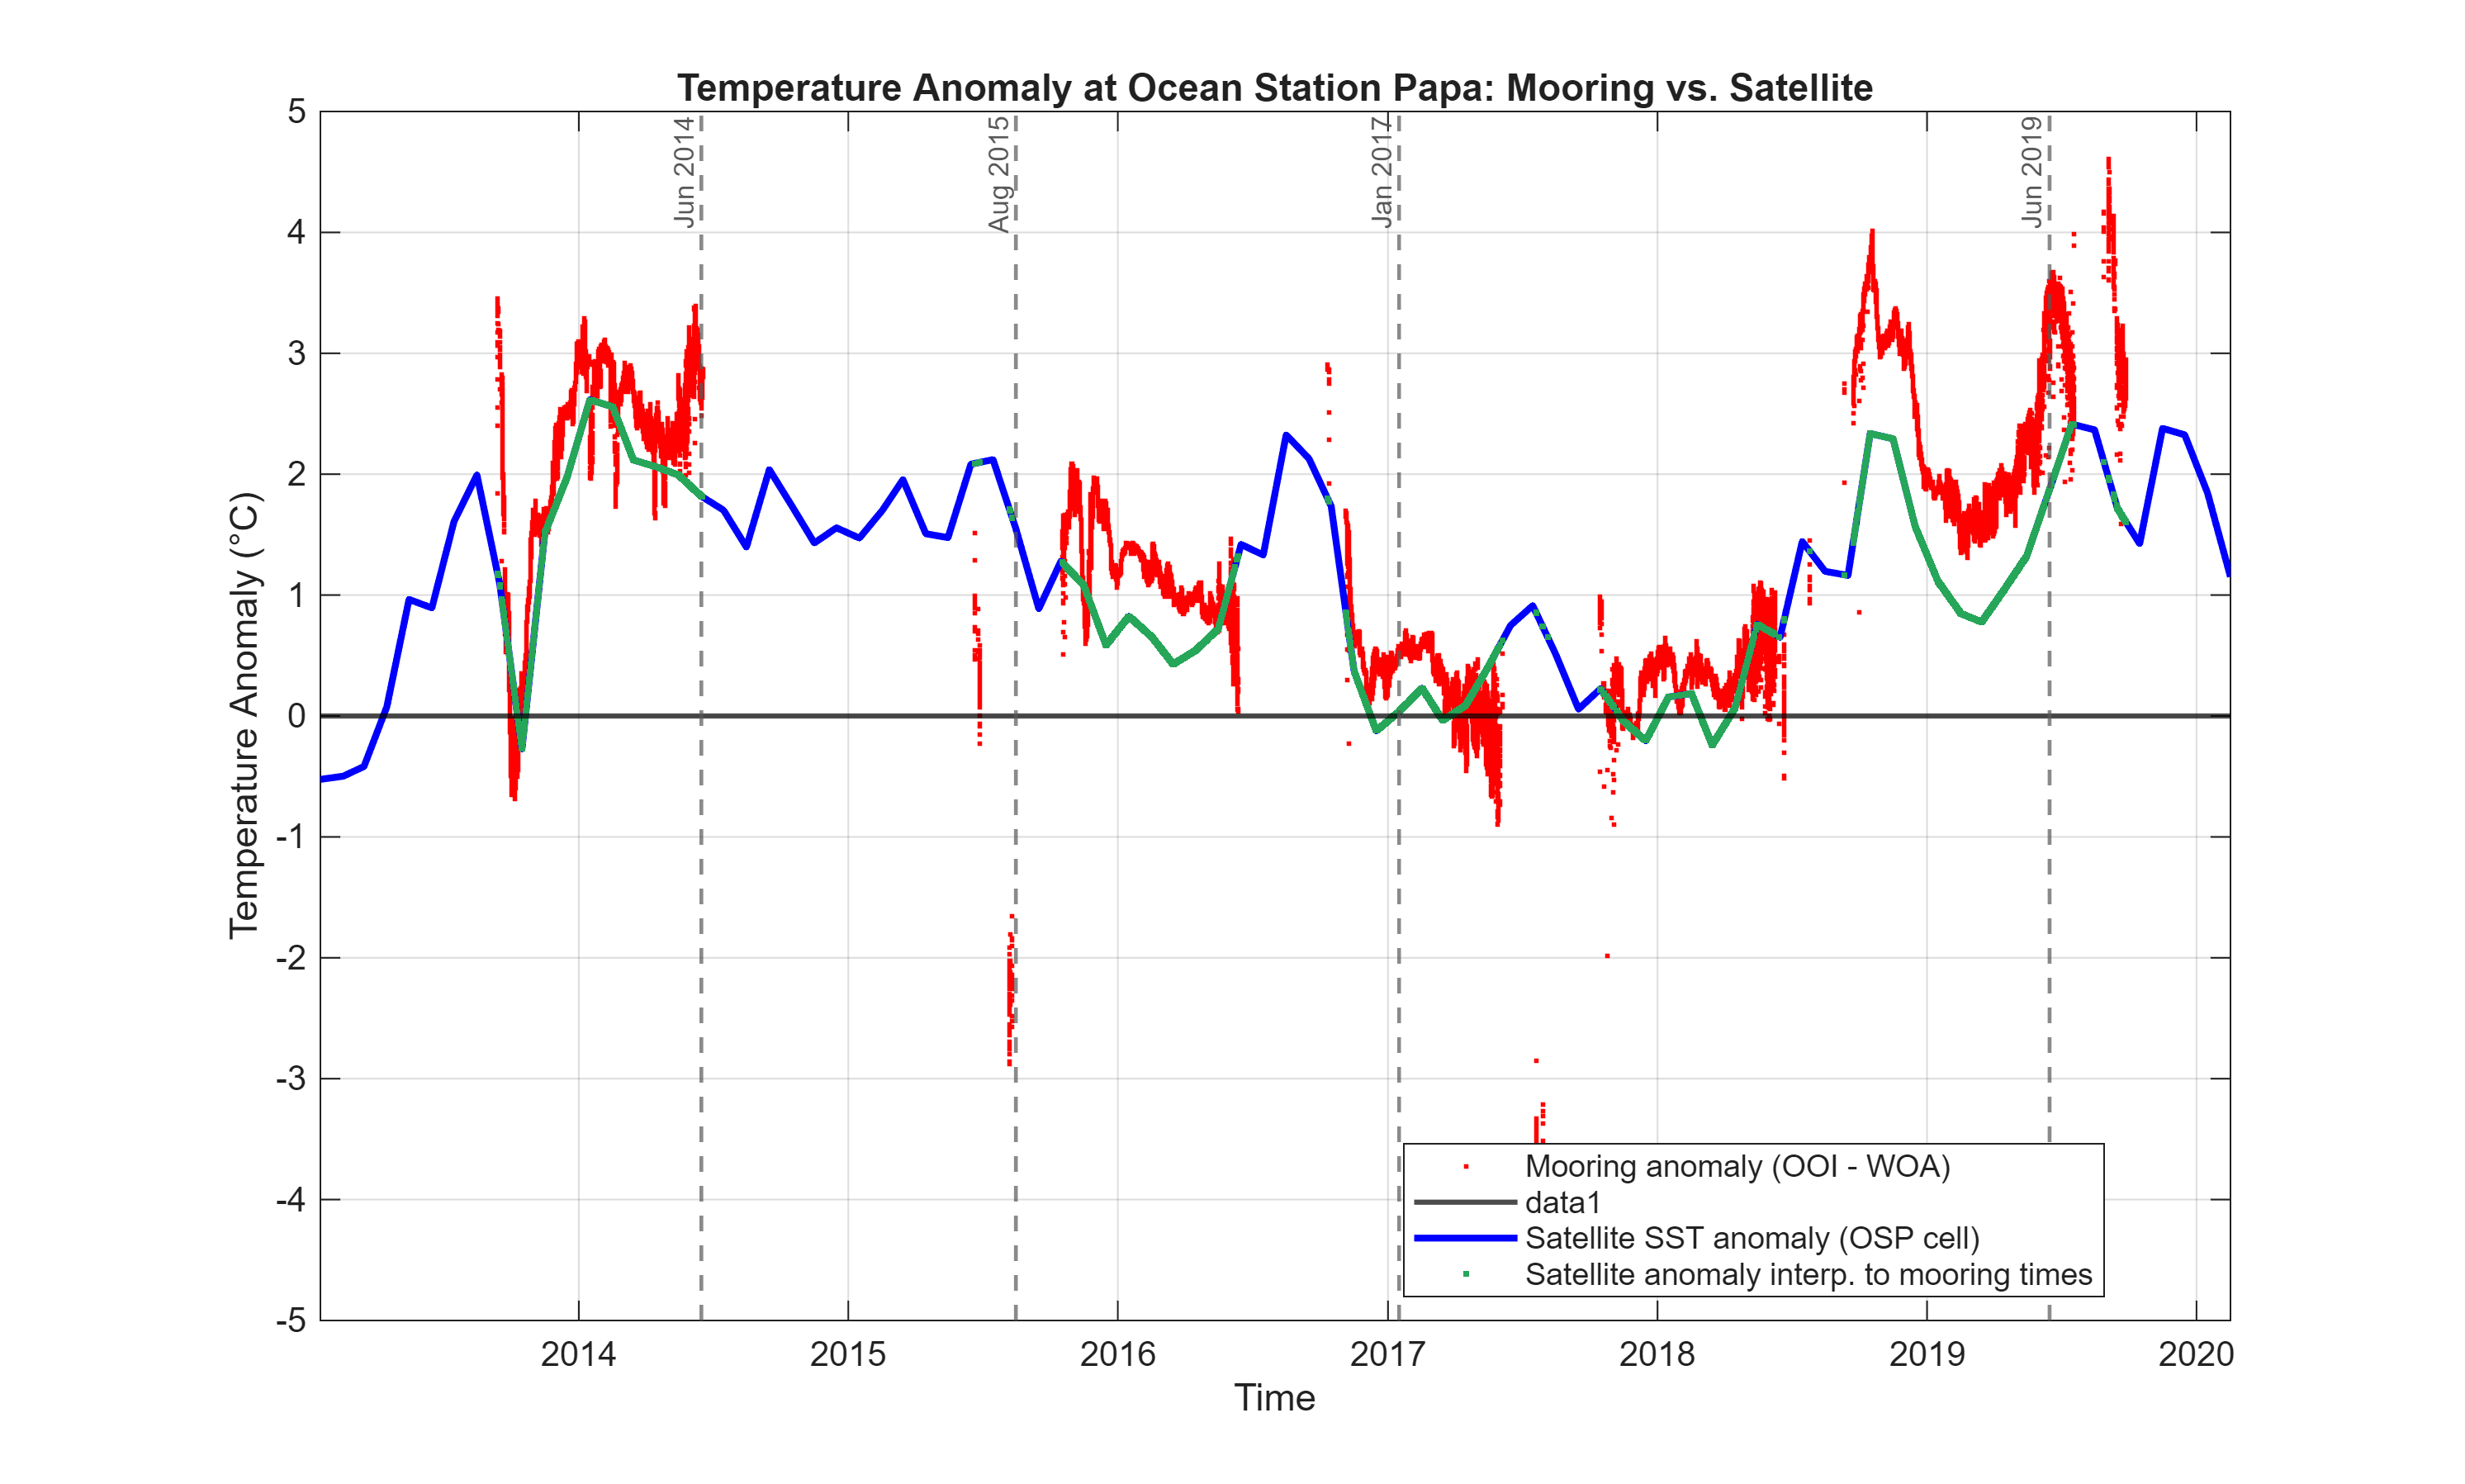
\includegraphics[width=0.95\textwidth]{figures/fig04_anomaly_compare.png}
  \caption{Temperature anomalies at OSP. Red points: $T'_{\mathrm{moor}}$ (mooring minus interpolated WOA climatology at \SI{30}{\meter}). Blue line: $T'_{\mathrm{sat,OSP}}$ from the MUR monthly \texttt{sstAnom} field (nearest grid cell; baseline MUR climatology 2003--2014). Green points: $T'_{\mathrm{sat,interp}}$ from Equation~(3) at each good mooring time. Gray vertical dashed lines mark the satellite months used for the maps in Figure~\ref{fig:maps}. Black horizontal line: zero anomaly.}
  \label{fig:anomaly_compare}
\end{figure}

Figure~\ref{fig:anomaly_compare} is the central comparison. The mooring anomaly traces warm and cool departures from the WOA seasonal template, including elevated values during the mid-2010s. The MUR SST anomaly at OSP (blue) is smoother in time (monthly) and tied to a different climatology than WOA, so overall bias and seasonally varying residuals relative to the red points are expected even when both capture the Blob. The green points show Equation~(3): they trace the monthly satellite curve but are sampled at mooring times for direct scatter-style comparison.

\begin{figure}[H]
  \centering
  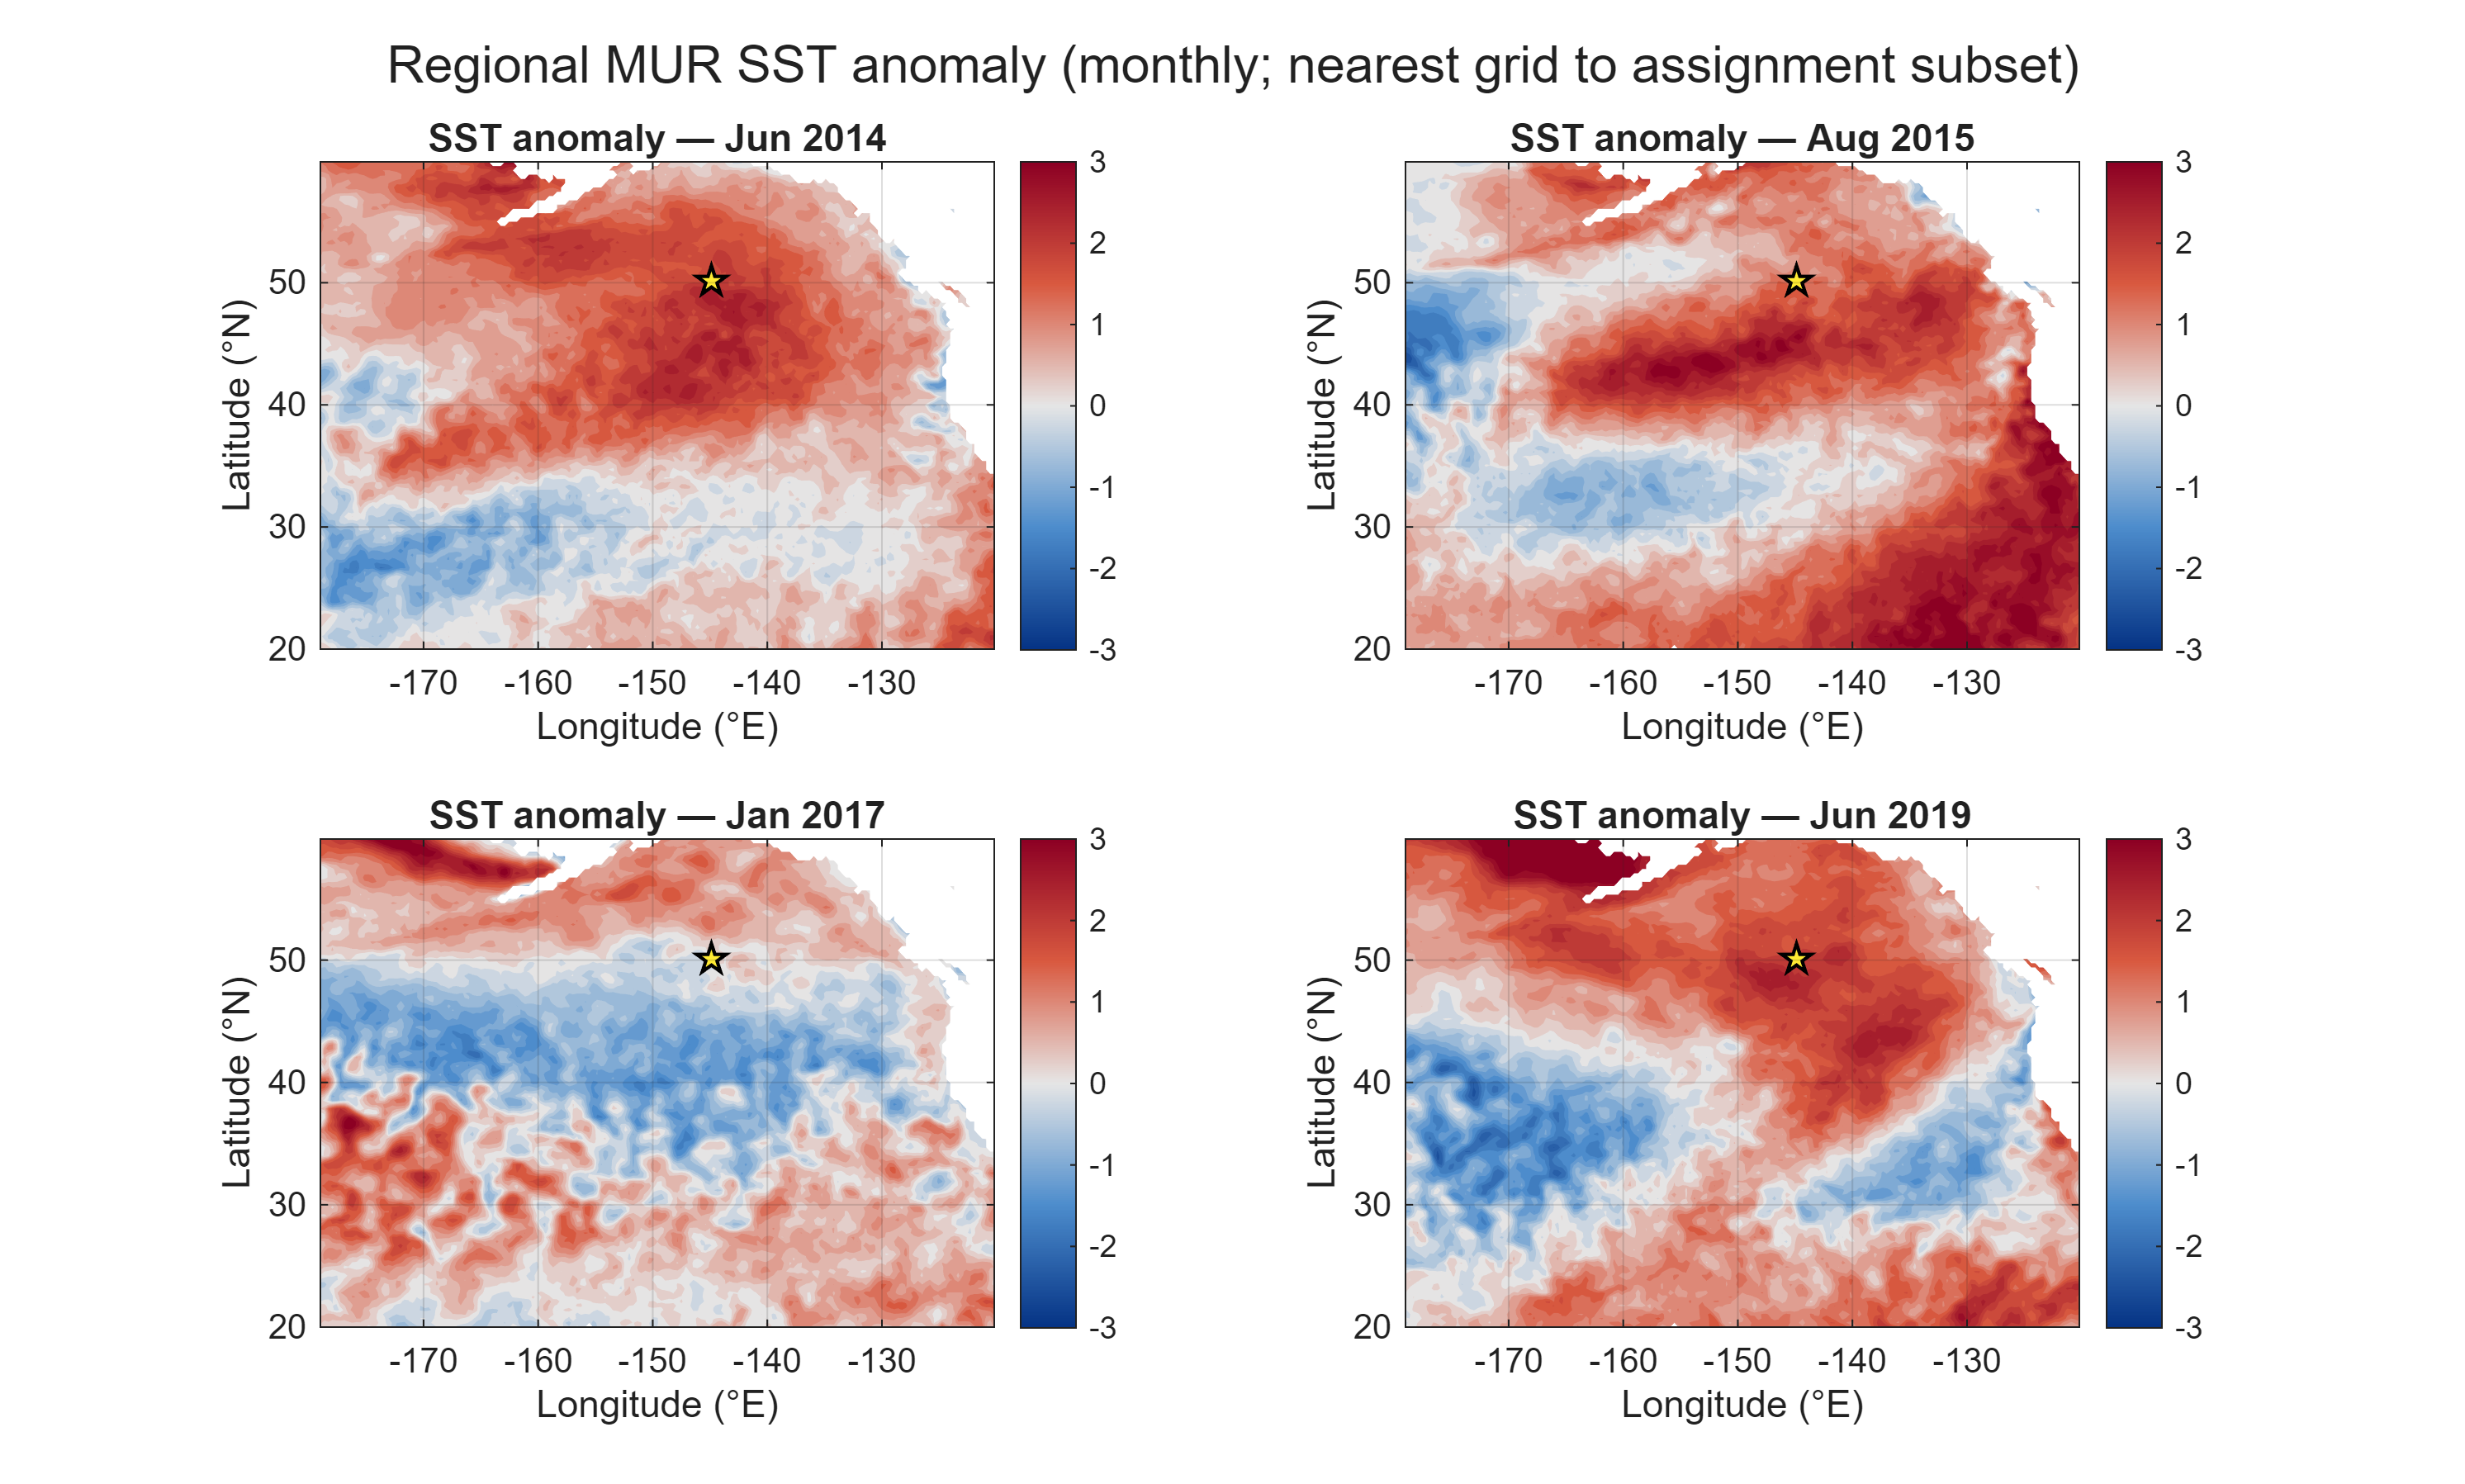
\includegraphics[width=0.95\textwidth]{figures/fig05_sst_anom_maps.png}
  \caption{Regional MUR monthly SST anomaly (\texttt{sstAnom}) for four months chosen within the OOI--satellite overlap (targets: June~2014, August~2015, January~2017, June~2019, each snapped to the nearest monthly file time). Filled contours use 25 evenly spaced levels from \SI{-3}{\degreeCelsius} to \SI{+3}{\degreeCelsius} (symmetric about zero) with a diverging colormap. Yellow marker: OSP. Together with Figure~\ref{fig:anomaly_compare}, the panels show whether warm anomalies at OSP coincide with basin-scale features or local gradients in the satellite field.}
  \label{fig:maps}
\end{figure}

Figure~\ref{fig:maps} (extension) places OSP inside the broader Northeast Pacific anomaly field. Warm anomalies during Blob years often extend over large zonal bands, but the exact pattern varies month to month; OSP can sit in regions of locally enhanced or weaker anomaly relative to the basin mean.

\subsection{Limitations of this analysis}
This study does not separate dynamical mechanisms (advection versus air--sea fluxes), does not quantify statistical significance of anomalies, and does not correct for sensor calibration drift. Monthly satellite sampling limits high-frequency comparison with the mooring. Using WOA for Equation~(2) and the MUR 2003--2014 baseline for Equation~(3) means the two anomaly series can disagree in mean and seasonal structure even when both reflect real ocean variability.

% ------------------------------------------------------------------
\section{Extensions completed}

\textbf{Extension 1 --- Visualizing data:} Following the lab prompt, I built a \textbf{multi-panel} set of regional \texttt{sstAnom} maps on the native MUR grid (Figure~\ref{fig:maps}), using four months spread across 2014--2019 within the mooring overlap. The same months are marked with vertical reference lines on Figure~\ref{fig:anomaly_compare} so readers can link the point anomaly time series to spatial context. Contour intervals are symmetric about zero (\SIrange{-3}{+3}{\degreeCelsius}), consistent with guidance for diverging climate maps.

\textbf{Extension 2 --- Reading scientific papers (6664):} I read Bond et al.\ \cite{bond2015} as context for the 2013--2015 northeast Pacific warm anomaly. Their overview of SST and atmospheric forcing motivates treating Figure~\ref{fig:maps} as snapshots of a coupled air--ocean event rather than isolated noise at one buoy.

% Undergraduate (4464): delete or replace Extension 2 if you only need one extension.

% ------------------------------------------------------------------
\section{Future work}

\subsection*{Other visualizations or calculations (same data)}
\begin{itemize}
  \item Co-locate WOA and satellite on the mooring grid by averaging mooring data to monthly means before computing $T'_{\mathrm{moor}}$ to match satellite resolution and reduce aliasing.
  \item Scatter plot of $T'_{\mathrm{moor}}$ versus $T'_{\mathrm{sat,interp}}$ with month-colored points to diagnose seasonal bias in residuals.
\end{itemize}

\subsection*{Re-doing the analysis with different methods}
\begin{itemize}
  \item Add daily MUR or NOAA OISST anomalies to resolve intra-month variability and compare correlation with the mooring at sub-monthly lags.
  \item Replace WOA with a recent climatology or a rolling baseline (e.g., 1981--2010 OISST climatology) so ``anomaly'' matches community practice for SST.
\end{itemize}

\subsection*{Additional data or context}
\begin{itemize}
  \item Add mixed-layer depth or SSH altimetry to test whether warm anomalies coincide with anomalous stratification or anticyclonic circulation.
  \item Incorporate atmospheric reanalysis (wind stress, net heat flux) to connect Figure~\ref{fig:maps} patterns to forcing as in Bond et al.\ \cite{bond2015}.
\end{itemize}

% ------------------------------------------------------------------
\section{Conclusions}
OOI temperatures at OSP track but exceed the WOA13 seasonal template during the mid-2010s warm period. Mooring anomalies (WOA baseline at \SI{30}{\meter}) and MUR SST anomalies (2003--2014 baseline at the surface) agree in broad timing for the Blob years but differ in detail because of depth, different climatologies, and monthly versus sub-monthly sampling. The extension maps show that OSP sits within evolving large-scale SST anomaly patterns rather than in isolation.

\begin{thebibliography}{99}
\bibitem{bond2015}
N.~A. Bond, M.~F. Cronin, H.~Freeland, and N.~Mantua, ``Causes and impacts of the 2014 warm anomaly in the NE Pacific,'' \emph{Geophysical Research Letters}, vol.~42, pp.~3414--3420, 2015.

\bibitem{hobday2016}
A.~J. Hobday \emph{et al.}, ``A hierarchical approach to defining marine heatwaves,'' \emph{Progress in Oceanography}, vol.~141, pp.~227--238, 2016.

\bibitem{locarnini2013}
R.~A. Locarnini \emph{et al.}, ``World Ocean Atlas 2013, Volume 1: Temperature,'' NOAA Atlas NESDIS 73, 2013.

\bibitem{chin2017}
T.~M. Chin, J.~V. Giglierano, and H.~H. Cheng, ``Multi-scale Ultra-high Resolution (MUR) Sea Surface Temperature (SST) Analysis Product,'' JPL publication, NASA MEaSUREs, 2017. Dataset: GHRSST Level 4 MUR Global Foundation SST, v4.1.
\end{thebibliography}

% ------------------------------------------------------------------
\newpage
\section*{Reflection}
\addcontentsline{toc}{section}{Reflection}

\textit{Instructions: Replace bracketed prompts with your own honest answers. If you submit the reflection only to your instructor by email, remove this section from the PDF you upload to Canvas.}

\paragraph{Transferable skills.}
\textbf{[Skill 1---e.g., multi-source data integration:]} [Describe what you practiced on this lab and how you would self-assess.]
\textbf{[Skill 2---e.g., visualization:]} [Same.]
\textbf{[Skill 3---e.g., scientific writing:]} [Same.]

\paragraph{Progress toward your SYOG goals.}
[State your goals for the course, whether they shifted after Data Lab \#2 feedback, and how this lab advanced them.]

\paragraph{Group experience.}
[Strengths and challenges of the group; your own contributions and growth edges; one lesson about collaboration you take away.]

\paragraph{Anything else.}
[Mention confusion you resolved, support you still want, or a rubric area where you would like detailed feedback, as invited in the syllabus.]

\end{document}
